\section{Background} \label{sec-background}
\subsection{Materialized View Selection}
In this section, we describe briefly describe the problem of materialized view selection and its relationship to our transformed dataset materialization.
\subsection{Hyperparameter Optimization}
In this section, we provide an overview of hyperparameter optimization techniques. 
Specifically, we first describe the grid search method.
Then we describe more advanced optimization methods and their heavy reliance on defining a proper search space and many iterations of search to acquire enough points to suggest good hyperparameter settings.

\subsection{Experiment Database}
A brief overview of the experiment databases, including several prior works such as OpenML and Schelter's  ML metadata management.

\subsection{Graph Representation of the Experiment Database}
\todo[inline]{This can also be moved to another chapter}
Description of how we will transform the experiment database into a graph.
Figure \ref{fig-graph-creation} shows the process of converting the experiment database into a graph.

\begin{figure}
\centering
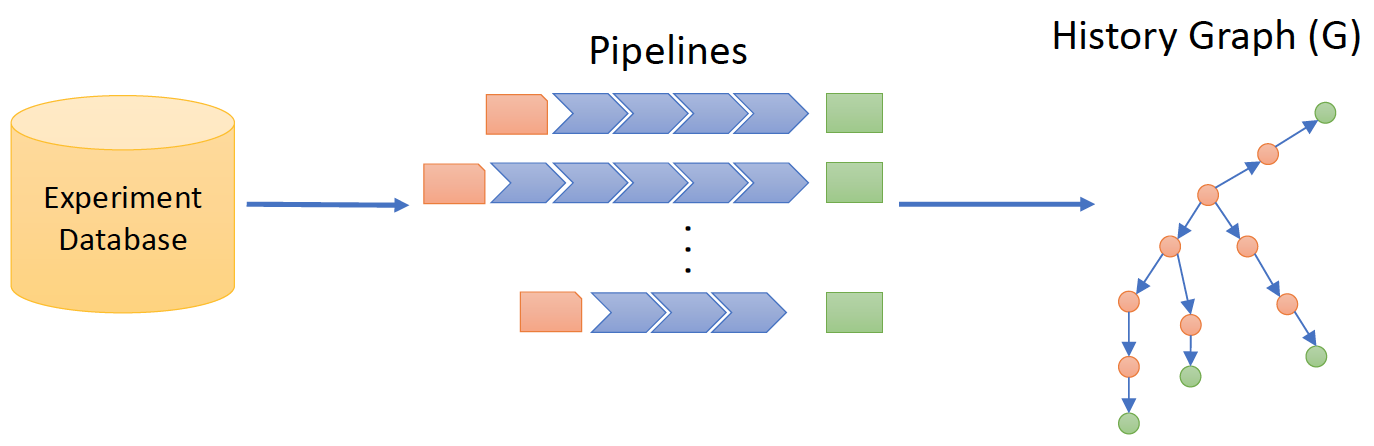
\includegraphics[width=\columnwidth]{../images/graph-creation.png}
\caption{Process of converting the experiment database to a graph}
\label{fig-graph-creation}
\end{figure}
